\documentclass[11pt]{beamer}
\usetheme{Warsaw}
\usepackage[utf8]{inputenc}
\usepackage[brazil]{babel}  % idioma
\usepackage{amsmath,amsfonts,amssymb,textcomp}
\usepackage{graphicx}
\usepackage{subfigure}

\usepackage[lined]{algorithm2e}

% Configurando layout para mostrar codigos C++
\usepackage{listings}
%\usepackage{minted}
%pdflatex -shell-escape minted01.tex
%ou
%latexmk -pdf -shell-escape minted01.tex

\author{ Othon Luiz Teixeira de Oliveira }
\title[PPGES]{Defesa da Dissertação de Mestrado}
%\setbeamercovered{transparent} 
%\setbeamertemplate{navigation symbols}{} 
%\logo{} 
\institute{Escola Politécnica de Pernambuco -- Poli ---  UPE} 
\date{29 - Maio - 2017} 
%\subject{} 
\begin{document}


\begin{frame}
	\titlepage
\end{frame}

% Capa - requer o TikZ
\newcommand{\capa}{
    \begin{tikzpicture}[remember picture,overlay]
        \node at (current page.south west)
            {\begin{tikzpicture}[remember picture, overlay]
                \fill[shading=radial,top color=orange,bottom color=orange,middle color=yellow] (0,0) rectangle (\paperwidth,\paperheight);
            \end{tikzpicture}
          };
    \end{tikzpicture}
}

%+++++++++++++++++++++++++++++++++++++++++++++++
\begin{frame}{PPGES}
	\begin{figure}[h]
		%\left
		
\includegraphics[width=16mm, height=13mm]{Figuras/Capa/upelogo.eps}
		\qquad \quad \quad \quad \quad
		
\includegraphics[width=17mm, height=15mm]{Figuras/Capa/logoPoli.jpg}
		\qquad \quad \quad \quad \quad \quad \quad 	\vspace{0.5in}
		
\includegraphics[width=20mm, height=15mm]{Figuras/Capa/icblogo.png}
		\\
		
\includegraphics[width=55mm, height=35mm]{Figuras/Capa/logo_ppges3.png}
		
	\end{figure}
\end{frame}

\begin{frame}\frametitle{ \Large Programa de Pós-Graduação em Engenharia de Sistemas}
	\begin{center}
		\Large \textbf{DISSERTAÇÃO DE MESTRADO} 
	\end{center}
	\pause
	\begin{block}
		\Large \textbf{Modelo Preditivo para Sugestão de Roteamento de cargas considerando dados históricos, sócio-ambientais, e de redes sociais}
	\end{block}
	
	\pause
	\vspace{0.3in}
	%\begin{block}
	\textbf{Mestrando:} Othon Luiz Teixeira de Oliveira \\
	\textbf{Orientador:} Prof. Dr. Fernando Buarque de Lima Neto
	%\end{block}
	
\end{frame}

%%% Colocando o sumário em cada início de sessão
\AtBeginSection[]{ 
	\begin{frame} 
		\frametitle{Sumário} \tableofcontents[currentsection] 
	\end{frame} 
} 

%+++++++++++++++++++++++++++++++++++++++++++++++
\section{ Introdução}
\subsection*{Introdução}


\begin{frame}\frametitle{Resumo}	
	\begin{block}{O cenário}
		\begin{itemize}
			\item O transporte de cargas no Brasil é feito principalmente pelas rodovias federais (BRs). 
			\pause
			\item Essas rodovias estão constantemente congestionadas nos perímetros urbanos.
			\pause
			\item Comunidades bloqueiam as rodovias para reivindicar, dos entes públicos, todo tipo de necessidades
			\pause
			\item Em alguns trechos o traçado das rodovias está próximo a morros e florestas.
		\end{itemize}
	\end{block}
\end{frame}

%--------------------------------------------------------
\section{ Objetivos}
\subsection*{ Principal}

\begin{frame}\frametitle{Proposição de um modelo preditivo}
	\pause
	\begin{block}{ Objetivo Geral}
		Esta pesquisa teve como principal objetivo desenvolver um modelo de plataforma autoadaptável 
		\pause que contemple predição do comportamento das rodovias federais pernambucanas,
		\pause antecipando alguns eventos que nela possam ocorrer, apontando onde ocorrerão.
		
	\end{block}
\end{frame}

\begin{frame}\frametitle{ Objetivos Específicos}
	\pause
	\begin{block}{ Quatro objetivos}
		\begin{itemize}
			\item Caracterizar a problemática de cada rodovia;

			\item Desenvolver um modelo preditivo dos fenômenos que envolvem as rodovias;

			\item Desenvolver um ambiente de simulações interativas da estrutura viária em sua dinâmica
			
			\item Propor soluções para melhorar a experiência dos usuários que utilizam as rodovias pernambucanas
		\end{itemize}
		
	\end{block}
\end{frame}

\begin{frame}\frametitle{PRF}
	%	\begin{block}{PRF & Twitter}
	\begin{itemize}
		\item Base de dados da Polícia Rodoviária Federal: acidente e interdições, entre 2007 a 2015.
		\pause
		\item Rede Social Twitter com 3200 tweets (limite permitido)
	\end{itemize}	
	%	\end{block}
\end{frame}

%++++++++++++++++++++++++++++++++++++++++++++++++++++++++++++++++++++++++++++++++++++++++++++++

\begin{frame}\frametitle{ Dados originais}
	\transboxin[duration=2, direction=25]	
	\begin{block}{ Planilha PRF}
		\begin{figure}[!ht]
			\centering %\centering % para centralizarmos a figura
			\caption{Planilha para Preprocessamento}
			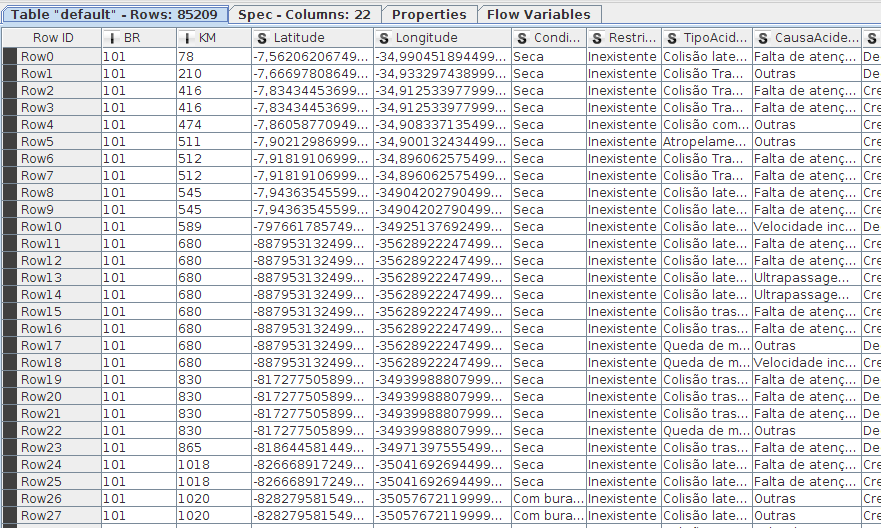
\includegraphics[width=110mm, height=40mm]{Figuras/BigData/PlanilhaPRF.png}
		\end{figure}
	\end{block}
\end{frame}


\begin{frame}\frametitle{ Entendendo a base de dados da PRF}
	\begin{exampleblock}{ Atributos e Instâncias -- iniciais}
		\begin{itemize}
			\item Dados de 2007 à 2015 -- BRs de Pernambuco
			\pause
			\item 85.209 Instâncias -- 27 Atributos
			\pause
			\item Dentre eles: Km, Latitude, Longitude, Condições da Pista, Causa do Acidente, Município, Data, Hora, Tipo de Veículo, 
			\pause
			\item Qtd de Feridos Graves,Qtd Feridos Leves, Qtd Mortos, Qtd Pessoas.
			
		\end{itemize}
	\end{exampleblock}
\end{frame}

\begin{frame}\frametitle{ O Tweeter}
	\begin{block}{ Acesso aos dados do Tweeter}
		\begin{figure}[!ht]
			\centering %\centering % para centralizarmos a figura
			\caption{Registro de App para para acessar e baixar dados}
			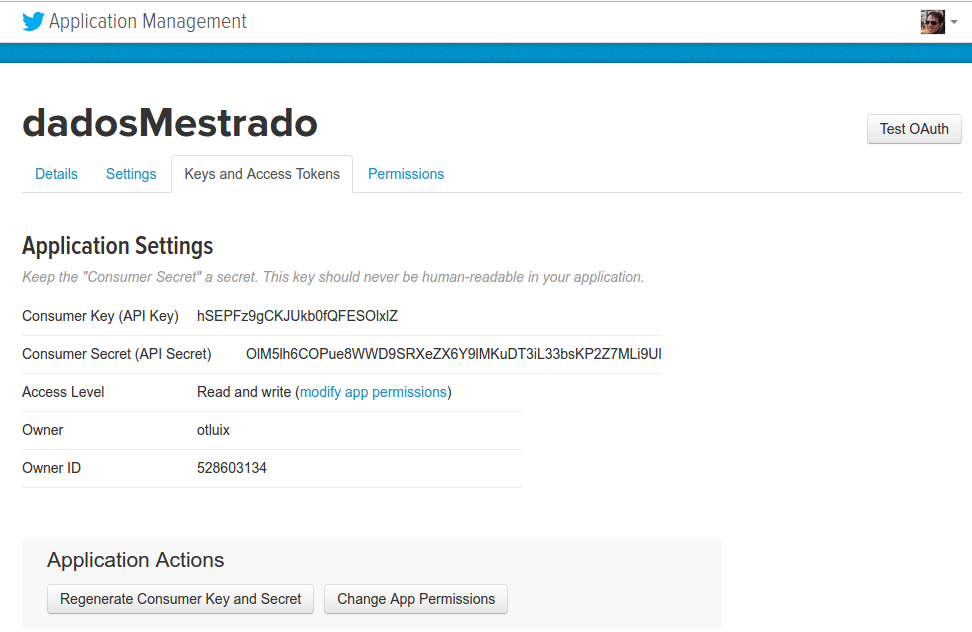
\includegraphics[width=80mm, height=35mm]{Figuras/BigData/appTweeter.png}
		\end{figure}
	\end{block}
\end{frame}

\begin{frame}\frametitle{ Dados originais}
	\transblindsvertical[duration=2, direction=25]
	\begin{block}{ Dados -- Planilha Tweeter}
		\begin{figure}[!ht]
			\centering %\centering % para centralizarmos a figura
			\caption{Planilha para Preprocessamento}
			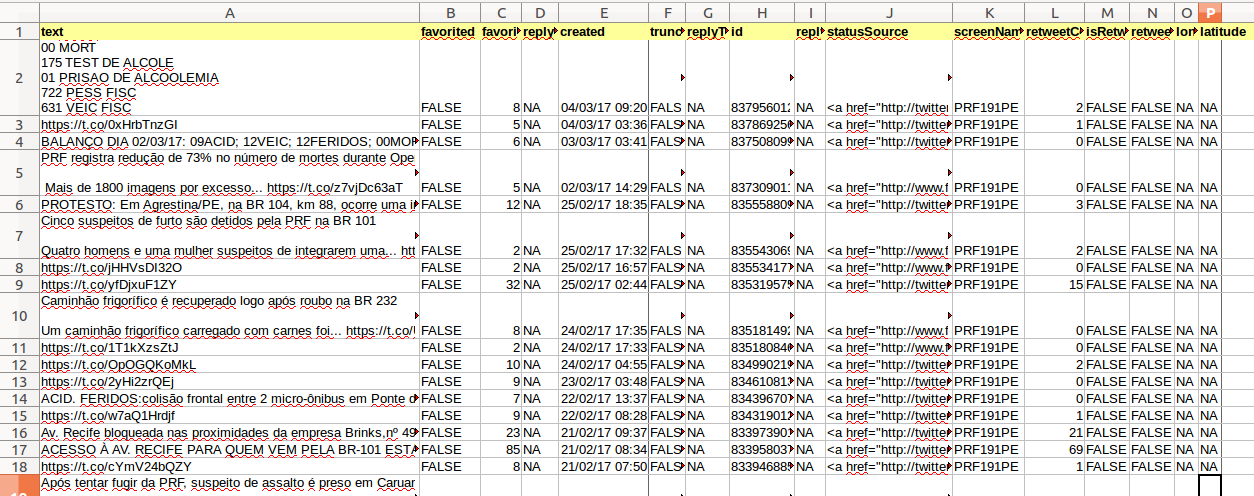
\includegraphics[width=110mm, height=40mm]{Figuras/BigData/tweetPRF.png}
		\end{figure}
	\end{block}
\end{frame}

\begin{frame}\frametitle{ Entendendo a base de dados do Tweeter}
	\begin{exampleblock}{Atributos e Instâncias -- iniciais}
		\begin{itemize}
			\item Dados de 2017 -- 2014 --- canal @PRF191PE
			\pause
			\item 2864 Instâncias -- 16 Atributos
			\pause
			\item Dentre eles: 'text, 'favorited', 'favoriteConunt', 'created', 'ID', 'statusSource', 'screenName', 'retweetCount',
			\pause
			\item 'isRetweet', 'retweeted', dentre outros.		
		\end{itemize}
	\end{exampleblock}
\end{frame}

%++++++++++++++++++++++++++++++++++++++++++++++++++++++++++++++++++++++++++++++++++++++++++++++

\section{ Metodologias de Mineração Dados}
\subsection*{ CRISP -- DM}

\begin{frame}\frametitle{ Domínio das técnicas de Mineração de Dados}
	\transdissolve[duration=2, direction=25]
	\begin{figure}[!ht]
		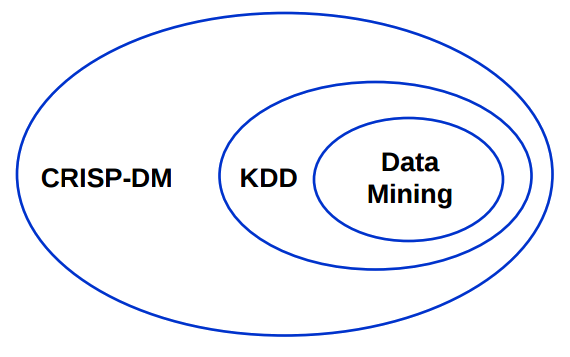
\includegraphics[width=90mm, height=60mm]{Figuras/BigData/RelacaoCrispKddDm.png}
	\end{figure}
\end{frame}


\begin{frame}\frametitle{ Cross Industry Standard Process for Data Maning -- CRISP - DM}
	\transboxout[duration=2, direction=25]
	\begin{figure}[!ht]
		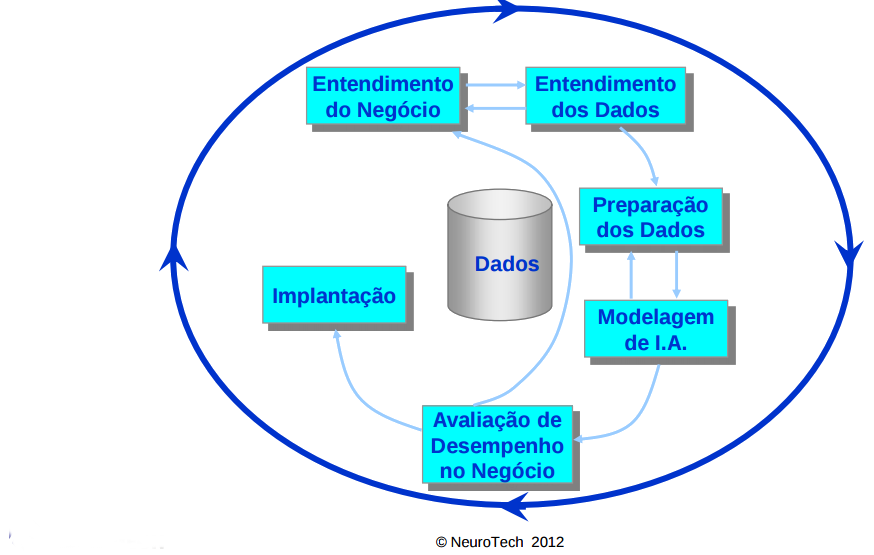
\includegraphics[width=90mm, height=60mm]{Figuras/BigData/CrispDM.png}
	\end{figure}
\end{frame}


\begin{frame}\frametitle{ Etapas CRISP-DM resumo}
	\transdissolve[duration=1, direction=25]
	\begin{figure}[!ht]
		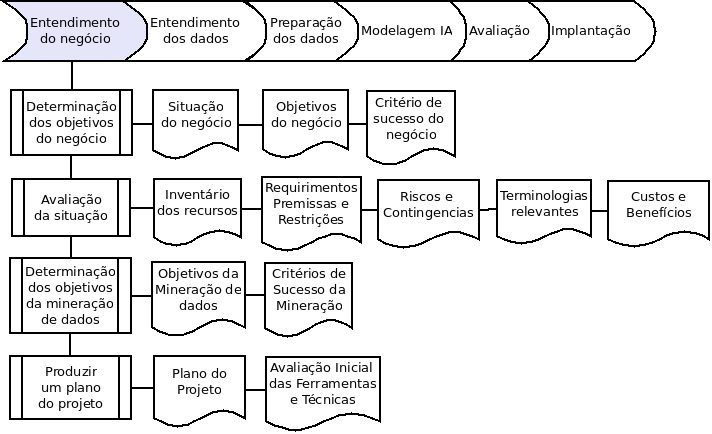
\includegraphics[width=80mm, height=58mm]{Figuras/Crisp/Entendimento.png}
	\end{figure}
\end{frame}

\begin{frame}\frametitle{ Etapas CRISP-DM resumo}
	\transdissolve[duration=1, direction=25]
	\begin{figure}[!ht]
		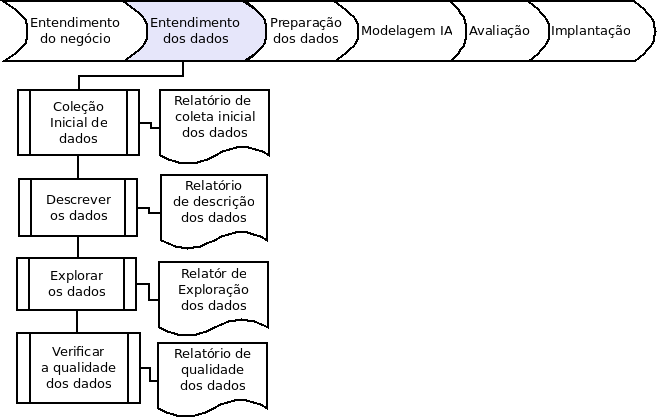
\includegraphics[width=80mm, height=58mm]{Figuras/Crisp/EntendDados.png}
	\end{figure}
\end{frame}

\begin{frame}\frametitle{ Etapas CRISP-DM resumo}
	\transdissolve[duration=1, direction=25]
	\begin{figure}[!ht]
		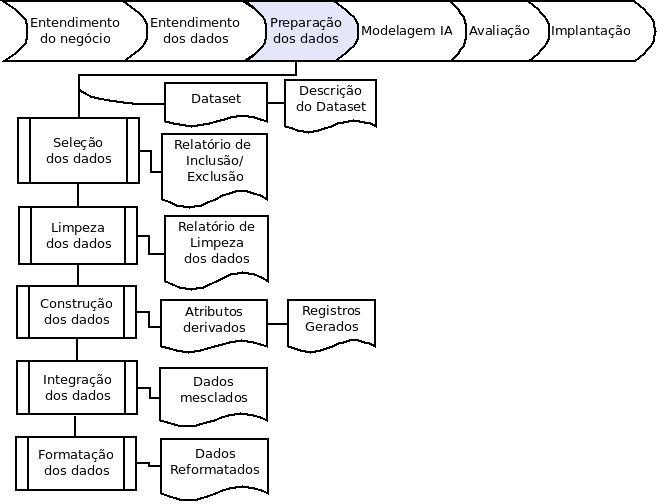
\includegraphics[width=80mm, height=58mm]{Figuras/Crisp/PreparaDados.png}
	\end{figure}
\end{frame}

\begin{frame}\frametitle{ Etapas CRISP-DM resumo}
	\transdissolve[duration=1, direction=25]
	\begin{figure}[!ht]
		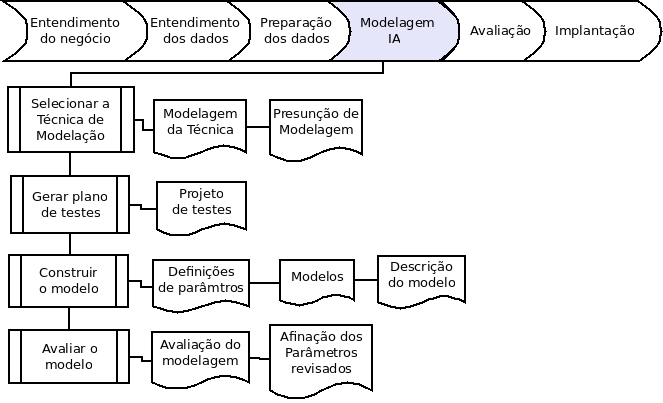
\includegraphics[width=80mm, height=58mm]{Figuras/Crisp/Model_IA.png}
	\end{figure}
\end{frame}

\begin{frame}\frametitle{ Etapas CRISP-DM resumo}
	\transdissolve[duration=1, direction=25]
	\begin{figure}[!ht]
		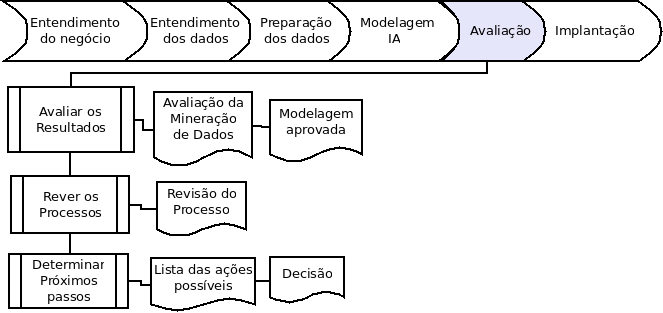
\includegraphics[width=80mm, height=58mm]{Figuras/Crisp/Avaliacao.png}
	\end{figure}
\end{frame}

\begin{frame}\frametitle{ Etapas CRISP-DM resumo}
	\transdissolve[duration=1, direction=25]
	\begin{figure}[!ht]
		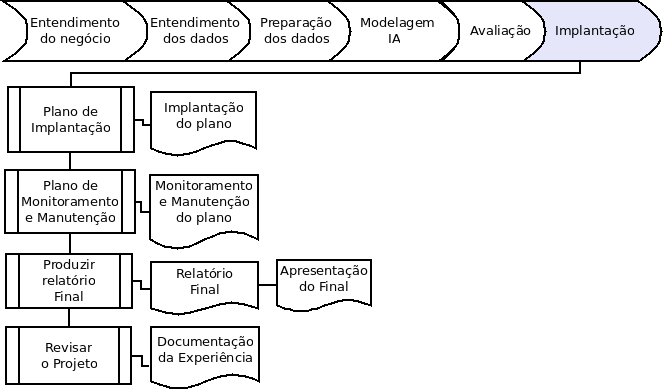
\includegraphics[width=80mm, height=58mm]{Figuras/Crisp/Implantacao.png}
	\end{figure}
\end{frame}

\section{KDD e Mineração de Dados}
\subsection*{ Minerando os dados do problema}

\begin{frame}\frametitle{ A descoberta de conhecimento (KDD) nas bases da PRF}
	\begin{figure}[!ht]
		%	\centering %\centering % para centralizarmos a figura
		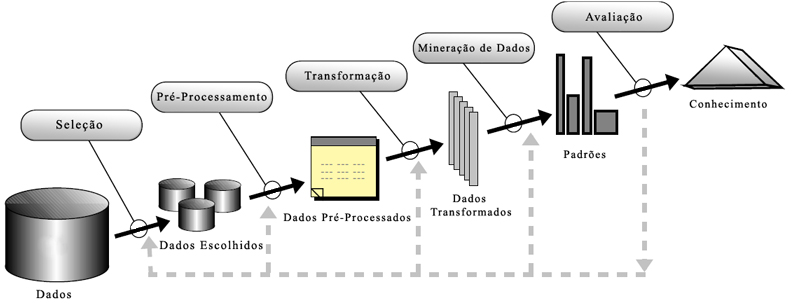
\includegraphics[width=100mm, height=30mm]{Figuras/BigData/Fayyad.png}
		\pause
		\begin{block}{ A base de dados original -- PRF}			
			40\% missing data -- 70\% do tempo total para tratar
		\end{block}
		\pause
		\begin{alertblock}{ Diferencça CRISP--DM --- KDD}			
			O CRISP-DM difere do KDD principalmente pelas fases do entendimento do  negócio (anterior ao KDD) e da implantação (posterior ao KDD)
		\end{alertblock}
	\end{figure}
\end{frame}


%++++++++++++++++++++++++++++++++++++++++++++++++++++++++++++++++++++++++++++++++++++++++++++++

\section{ Tecnologias empregues na Mineração Dados}
\subsection*{ Árvore de Decisão}

\begin{frame}\frametitle{ Domínio das técnicas de Mineração de Dados}
	\transdissolve[duration=2, direction=25]
	\begin{figure}[!ht]
		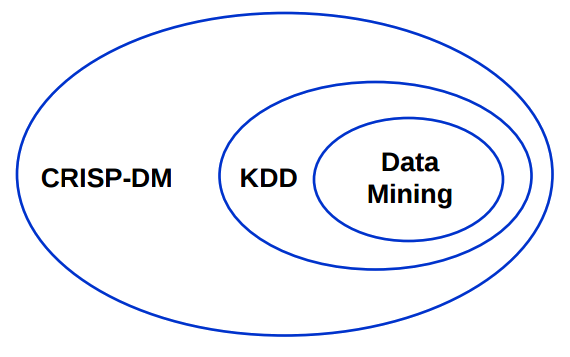
\includegraphics[width=90mm, height=60mm]{Figuras/BigData/RelacaoCrispKddDm.png}
	\end{figure}
\end{frame}


\subsection*{ Naïve Bayes}

\begin{frame}\frametitle{ Domínio das técnicas de Mineração de Dados}
	\transdissolve[duration=2, direction=25]
	\begin{figure}[!ht]
		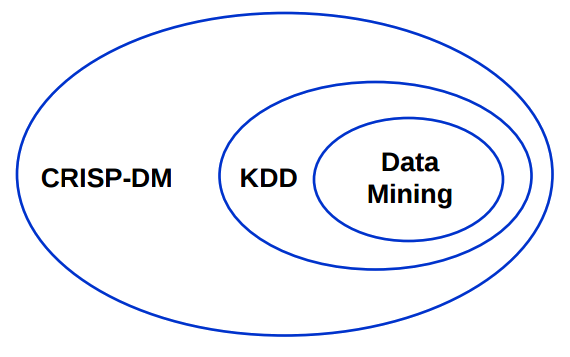
\includegraphics[width=90mm, height=60mm]{Figuras/BigData/RelacaoCrispKddDm.png}
	\end{figure}
\end{frame}

\subsection*{ Redes Neurais}

\begin{frame}\frametitle{ Domínio das técnicas de Mineração de Dados}
	\transdissolve[duration=2, direction=25]
	\begin{figure}[!ht]
		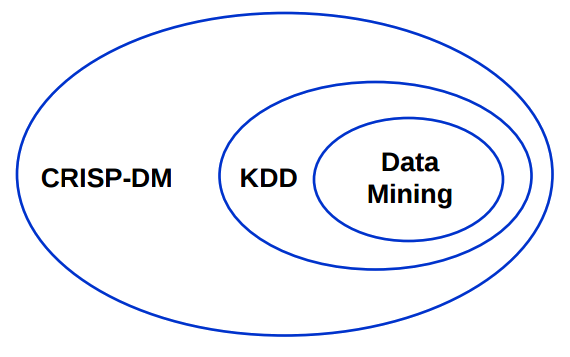
\includegraphics[width=90mm, height=60mm]{Figuras/BigData/RelacaoCrispKddDm.png}
	\end{figure}
\end{frame}

%++++++++++++++++++++++++++++++++++++++++++++++++++++++++++++++++++++++++++++++++++++++++++++++

\section{ Mineração em Textos}
\subsection*{ Tecnologias empregues na Mineração em Textos}

\begin{frame}\frametitle{ TF -- IDF}
	\transdissolve[duration=2, direction=25]
	\begin{figure}[!ht]
		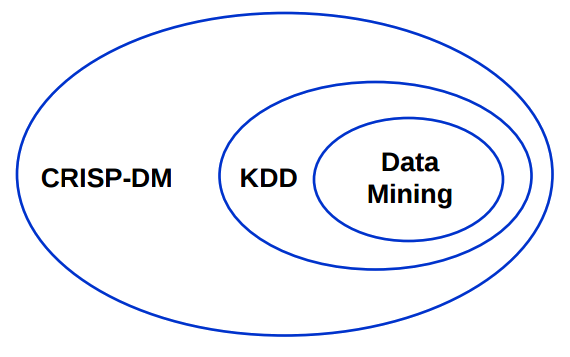
\includegraphics[width=90mm, height=60mm]{Figuras/BigData/RelacaoCrispKddDm.png}
	\end{figure}
\end{frame}


\begin{frame}\frametitle{ K-means para Agrupamentos dos dados}
	\transdissolve[duration=2, direction=25]
	\begin{figure}[!ht]
		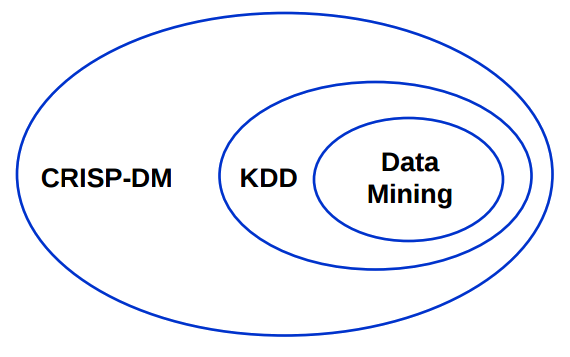
\includegraphics[width=90mm, height=60mm]{Figuras/BigData/RelacaoCrispKddDm.png}
	\end{figure}
\end{frame}

%++++++++++++++++++++++++++++++++++++++++++++++++++++++++++++++++++++++++++++++++++++++++++++++

\section{ Trabalhos Futuros}
\begin{frame}\frametitle{Trabalhos futuros}
\transboxout[duration=2, direction=25]
	\begin{figure}[ht]
		\centering
		\caption{ Interface Gráfica Proposta}
		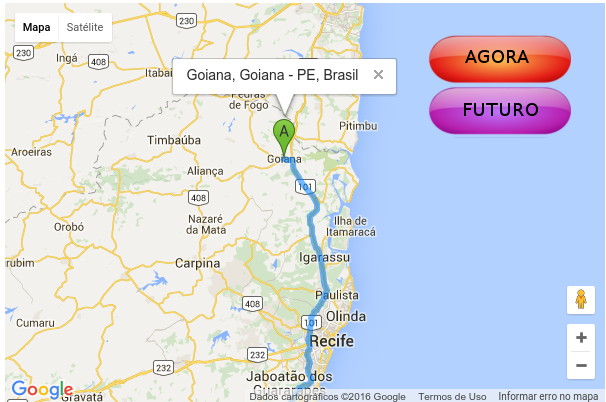
\includegraphics[width=100mm, height=45mm]{Figuras/BigData/InterfaceGrafica.png}
	\end{figure}
	
\end{frame}

\end{document}
